\documentclass[a4paper,titlepage,11pt]{article}

\usepackage[utf8x]{inputenc}
\usepackage{graphicx}

\begin{document}

\begin{titlepage}
  \begin{center}
    {\scshape \huge Truthful Emergencies \par}
    \vspace{1cm}

    {\scshape \LARGE Proposal \par}
    \vspace{1.5cm}

    {\scshape \Large Network and Computer Security \par}
    \vspace{0.5cm}

    {\Large Alameda \par}
    \vfill

    {\itshape \Large Group 11 \par}
    \vfill

    \begin{tabular}{l l l}
      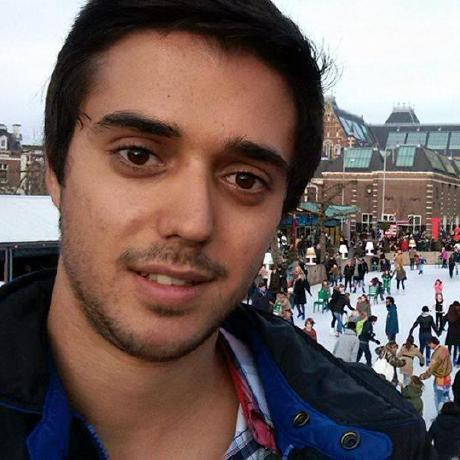
\includegraphics[width=10mm, height=10mm]{img/bernardo.jpeg} & Bernardo Casaleiro & 87827\\
      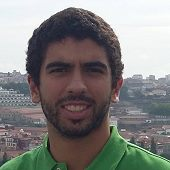
\includegraphics[width=10mm, height=10mm]{img/joao.jpeg} & João Godinho & 87830\\                       % TODO change the photo
      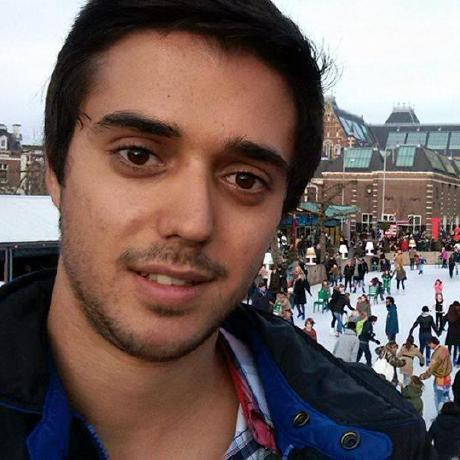
\includegraphics[width=10mm, height=10mm]{img/bernardo.jpeg} & Miguel Pinto & nnnnn\\                       % TODO change the photo and student number
    \end{tabular}
    \vfill

    {\large \today\par}
  \end{center}
\end{titlepage}

\section{Problem}
First response emergency systems are a limited resource. Their usage makes a difference in life-or-death situations!

Requesting an ambulance is a serious matter.
It should be simple, secure, fast and first of all always available.
For that the Dispatch Center must be fault tolerant.

It should separate the real requests from the false ones and provide a response accordingly.
Improper usage must be punished while real requests should trigger an appropriate response.

\section{Requirements}

\subsection{Application Requirements}
\begin{enumerate}
  \item Send a request of an emergency.
  \item Consult the expected time for the request to be answered.
\end{enumerate}

\subsection{Server Requirements}
\begin{enumerate}
  \item Insert a request in a queue depending on the user rating.
  \item Log the requests.
  \item Send the expected time of response to the user
  \item Send the confirmation that an ambulance is en route.
  \item Rate the user accordingly at the end of the request.
  \item Block a user for abusive usage.                                                         % TODO review
\end{enumerate}

\subsection{Security Requirements}
\begin{enumerate}
  \item Non-repudiation.
  \item Fault tolerance to DoS.
  \item Firewall, responsible for filtering the requests.
  \item Auditing mechanisms.
  \item Secure channel between user and Dispatch Central.
\end{enumerate}

\subsection{Non-functional Requirements}
Our main goal is to build a secure application, not forgetting that in real life,
our service couldn't be slow due to the fact that time in an emergency situation is crucial.

\section{Proposed solution}

\begin{center}
  \textit{What's the cost of a human life?}
\end{center}

There's no perfect solution and everything breaks eventually.
Our goal is to make it harder to break with the time and money we have at our disposal.
So with this in mind we design this solution.

\subsection{Basic solution}
In this solution we assume that the communications between the User and the Dispatch Central are secure.
The main goal of this sprint is to build the foundation and the architecture to facilitate the implementation of the security parts.

There are no keys or certificates involved in this step so non-repudiation will not be our goal here.

We will have a centralized Dispatch Central that will receive all the requests from the Users.

Auditing mechanisms will be considered in this phase and for that we will use logs on the Central side.
Everytime a request is received it is registered in a log for the auditing personal be able to review.
Each entry will have a timestamp and the contents of the message (ID, Location, Situation).

After processing the request, and approving it, the Dispatch sends the confirmation message that an ambulance is on the way.
Otherwise the user will be accounted for the incorrect usage and warned of the possible consequences of further reckless behavior.

\subsection{Intermediate solution}
In this phase, we will create manually all the keys and certificates\footnote{self-signed}.

Each entity will have his own set of keys, but the certificates will have to be requested to the CA by the user to get his public key.        % TODO review
This will give a structure to implement non-repudiation taking the assumption that the private keys are never stolen
by some sort of malware or someone accessing the machine physically.

Each message sent by the user will be signed with his own private key.
With the previous assumption we can guarantee that the user sending the message was really him.

The Dispatch Central will retrieve the user public key from the certificate that was requested after receiving and deciphering the message.   % TODO review
The procedure is the same for the message flow from the Dispatch to the user.

\subsection{Advanced solution}
On this last phase of the project, we will focus on fault tolerance on the primary server (DoS, crash, etc.).
We will also focus in building a firewall responsible for detecting bad or duplicate requests,
redirecting connections to secure ports and analyzing packet contents.

\section{Tool references}

\section{Work Plan}
To facilitate, we will divide the project according to the requirements.

Example: b\_2.2.2 means Basic job on Server Requirement(2.2) - "Log the requests"(1). 

The jobs might be basic(b), intermediate(i) or advanced(a).
\begin{center}
    \begin{tabular}{| l || l | l | l |}
    \hline
    Week Start & Miguel & Bernardo & João \\ \hline \hline
    24 Out & a & b & c \\
    31 Out & a & b & c \\
    7 Nov & a & b & c \\
    14 Nov & a & b & c \\
    21 Nov & a & b & c \\ 
    28 Nov & a & b & c \\ 
    5 Dez & a & b & c \\ \hline

    \end{tabular}
\end{center}

\end{document}
